\chapter{Language design}\label{cha:languagedesign}
This chapter prioritizes Arc's characteristics based on the criteria from~\cite{Sebesta2016}, and briefly covers the lexer and parser generator tools: JavaCC, \gls{antlr}, and JFlex with Cup, that were considered for the project.

The language specification consisting of the syntax, contextual constraints, and semantics, is also covered in this chapter. Section~\ref{sec:syntax} covers Arc's \gls{cfg} and a description of Arc's types, structures, and constructs. Section~\ref{sec:contextualconstraints} details the scope rules and the type rules, which make up the contextual constraints. Lastly, section~\ref{sec:languagesemantics} outlines the important parts of the semantics.

\section{Language criteria}\label{sec:languageeval}
There is no common consensus on objectively evaluating a language. The measurement of compilation speed, execution speed, and file size, address the efficiency of the language's implementation, not the language's design. Popularity could be measured but would vary significantly with time and contain several skews from bias. Popularity also does not necessarily mean that a language is generally good; for example, English is popular, but it is also a very ambiguous language.

As such, a set of prioritized language evaluation criteria has been determined based on the criteria presented in~\cite{Sebesta2016}. An objective evaluation of the language based on these criteria is not practically possible~\cite{Sebesta2016}; however, the criteria may work well when making decisions during language design, implementation, and evaluation. This section presents the most relevant concerns regarding the choice of relevant criteria.

The primary concern is with the programming language users - writers of Arduino programs - in this case, the Arduino hobbyist. The programming of an Arduino project may be secondary to hobbyists, who prioritize the hardware aspects of their project.

The secondary concern is the concurrency issue that follows from the primary concern - making an Arduino behave concurrently is not a trivial programming task. There are several available options to implement concurrency, but each with different issues, and none solve the issue in a general way~\cite{Restucia2022}.

The tertiary and last concern follows from the secondary issue - determining how to use concurrency to solve the problem in an Arduino. Concurrency problems can be subtle and complex, so understanding that it is even a  concurrency issue may not be immediately apparent. Thus a simple solution may be hard to spot.


\subsection{Criteria and characteristics}\label{subsec:priorityofcriteria}
Table~\ref{tab:langevalcrit} lists many characteristics that a programming language might want and their impact criteria. Sebesta~\cite{Sebesta2016} lists four criteria: readability, writability, reliability, and cost. These criteria are affected by several characteristics with varying influence and importance~\cite{Sebesta2016}. It is important to note that while these characteristics can not be measured, they are essential to keep in mind when designing the language.


\begin{table}[htb!]
    \centering
    \begin{tabular}{lccc}
        \toprule
                                & \multicolumn{3}{c}{CRITERIA}                                               \\
        \textbf{Characteristic} & \textit{Readability}         & \textit{Writability} & \textit{Reliability} \\
        \cmidrule(r){2-4}
        Simplicity              & \textbullet                  & \textbullet          & \textbullet          \\
        Orthogonality           & \textbullet                  & \textbullet          & \textbullet          \\
        Data types              & \textbullet                  & \textbullet          & \textbullet          \\
        Syntax design           & \textbullet                  & \textbullet          & \textbullet          \\
        Support for abstraction &                              & \textbullet          & \textbullet          \\
        Expressivity            &                              & \textbullet          & \textbullet          \\
        Type checking           &                              &                      & \textbullet          \\
        Exception Handling      &                              &                      & \textbullet          \\
        Restricted Aliasing     &                              &                      & \textbullet          \\
        \bottomrule
    \end{tabular}
    \caption{The three main criteria and the related characteristics~\cite{Sebesta2016}.}
    \label{tab:langevalcrit}
\end{table}


\subsubsection{Readability}
Readability describes how easy programs can be read and understood\cite{Sebesta2016}. The importance of readability is evident in the maintenance of programs, where programs with low readability are complicated and overwhelming to read.

\subsubsection{Writability}
Writability describes how easy a program is to write~\cite{Sebesta2016}. A language with good writability allows writers to express their intent more easily.

\subsubsection{Reliability}
Reliability describes how reliable a program is~\cite{Sebesta2016}. Reliability is essential, as a highly reliable program will perform correctly under all conditions.

\subsubsection{Cost}
The cost is described as a combination of several factors, such as teaching new programmers to use the language and the cost of writing the language. These costs all add up, and many things reduce this cost, such as better readability and writability, faster compile times, better reliability, and more~\cite{Sebesta2016}.

\subsection{Priority of characteristics by importance}
With these considerations in mind, we have prioritized and selected the characteristics for each criterion as we expect them to matter in this context.

The primary concern deals with considerations related to the cost criterion. Specifically, the cost associated with learning and understanding the programming language is essential. This consideration suggests that general simplicity, in the form of few but expressive language constructs and precise, consistent combination and application of the constructs is \textbf{very important}. It may also be problematic because concurrency is a complex topic.

Syntax design is also a \textbf{very important} characteristic, as seen from the secondary and tertiary concerns. The language should concisely express new constructs that are not available in the Arduino language. An aim of the syntax could be to use well known notation and keywords.

Data types are probably also an \textbf{important} characteristic. As long as the expressivity of the language is not significantly affected, the amount of data types is reduced by generalizing them. An example of this would be data types such as integers, doubles, and floats, all generalized to a single data type. Compared to the Arduino language, this reduction of data types is likely to affect overall simplicity and writability positively, and therefore cost, which is essential to hobbyists. This characteristic is also related to orthogonality - having fewer constructs and a consistent rule set for combining them is often better than having many primitives. Orthogonality is therefore also an \textbf{important} characteristic.


Expressivity is only \textbf{somewhat important} since concurrency language constructs are an aim of the language. Having too few data types is likely to harm the simplicity of the language since some things would take more work to express. On the other hand, good support for abstraction through user-defined types may enable advanced users to have greater freedom. However, readability is more important to learning than writability, and support for abstraction is \textbf{not important}.

Type checking at compile-time, especially concurrency-related issues, such as mutability, would potentially be compelling, but it depends on the rest of the design. For now, it is \textbf{less important}.

Arduino does not use the exceptions and exception handling available in the C++ language by default. The standard solution for Arduino code writers is to write code that handles the possible exceptions that may occur without the exception language constructs. For the sake of footprint, this will also be the preferred solution for this project, and exception handling is \textbf{not important}.

Aliasing refers to having two or more distinct names in a program that refers to the same memory location~\cite{Sebesta2016}. The simpler the language is, for example, not having pointers, the easier this is to restrict. While restricted aliasing is \textbf{very important}, it is expected to be easy to manage in a simple language. When dealing with concurrency, it is also essential to avoid accidental data corruption.


\begin{table}[htb]
    \centering
    \begin{tabular}{l>{\centering}p{2cm}>{\centering}p{2cm}>{\centering}p{2cm}>{\centering\arraybackslash}p{2cm}}
        \toprule
        \textbf{Characteristics}    &
        \textbf{Very important}     &
        \textbf{Important}          &
        \textbf{Somewhat important} &
        \textbf{Not important}                      \\ \midrule
        Simplicity                  & X &   &   &   \\
        Orthogonality               &   & X &   &   \\
        Data types                  &   & X &   &   \\
        Syntax design               & X &   &   &   \\
        Support for abstraction     &   &   &   & X \\
        Expressivity                &   &   & X &   \\
        Type checking               &   &   & X &   \\
        Exception handling          &   &   &   & X \\
        Restricted aliasing         & X &   &   &   \\
        \bottomrule
    \end{tabular}
    \caption{Summary of the characteristics and their importance.}
    \label{tab:priorityofcharacteristics}
\end{table}


It is worth noting that the Arduino programming language already has addressed several of the above concerns compared to C++. Examples of this can be seen in introducing new constants and the disabling of some language capabilities like exceptions and try-catch blocks from C++. The Arduino IDE is another point to consider in favor of cost concerns for the Arduino platform.

\section{Parser generator}\label{sec:parsergenerator}
For generating code and parsing, based on a grammar, there exists many tools to do this automatically. Therefore, a discussion of \textit{JavaCC}, \textit{ANTLR4}, and \textit{CUP} precedes the formal language description. The tools mentioned are only a few of those available and have been chosen because the group has experience with them through coursework.  The main reason a parser generator has been chosen is because of the gains in productivity that it makes possible. It also makes it possible to create a functioning compiler yet still have language design as a larger focus.

Each tool is evaluated using a reduced fragment of the Bims grammar from Table~\ref{tab:bimsgrammar}~\cite{Huttel2010}. For each tool, the grammar was adapted, and the tool was run with the rewritten grammar as input. The process of rewriting, inputting, and running the tool was compared, and a tool was selected.


\begin{table}[htb!]
  \centering
  \begin{tabular}{l}
    $n \in \textbf{Num} - \text{Numerals}$                \\
    $x \in \textbf{Var} - \text{Variables}$               \\
    $a \in \textbf{Aexp} - \text{Arithmetic expressions}$ \\
    $b \in \textbf{Bexp} - \text{Boolean expressions}$    \\
    $S \in \textbf{Stm} - \text{Statements}$              \\
  \end{tabular}
  \begin{align*}
    S & \rightarrow x \coloneqq a \mid \text{skip} \mid S_1;S_2                          \\
    b & \rightarrow a_1 = a_2 \mid a_1 < a_2 \mid \neg b_1 \mid b_1 \land b_2 \mid (b_1) \\
    a & \rightarrow n \mid a_1 + a_2 \mid a_1 * a_2 \mid a_1 - a_2 \mid (a_1)
  \end{align*}
  \caption{Sample Bims syntax \cite{Huttel2010}}
  \label{tab:bimsgrammar}
\end{table}


\subsection{JavaCC}
JavaCC stands for Java Compiler Compiler and is an open-source parser generator and lexical analyzer developed by Oracle, written in the Java language. It is one of the most popular parser generators for Java~\cite{JavaCC2021}, and it is very well documented.

JavaCC takes as input a Context-Free Grammar (CFG) in Extended Backus-Naur Form (EBNF) to generate a scanner and a parser based on the input. The parser generated is a Left-to-right, Leftmost derivation with 1 token lookahead (LL(1)) parser by default. However, the parser can be extended to \textit{k} lookahead for parts of the grammar if necessary~\cite{JavaCC2021}.

Setting up JavaCC was easy as it is well documented, and requires Java to be installed. Having set this up, we were able to begin writing our grammar. After setting up, it became clear that writing grammars in JavaCC is simple but a bit hard to read. In JavaCC, the grammar has to be written as code, whereas the syntax of other tools resembles the way it is seen in books, as shown in Table~\ref{tab:bimsgrammar}. An example of this can be seen in Listing~\ref{List:javaCC}

\begin{listing}[htb!]
  \centering
  \begin{minted}{java}
    PARSER_BEGIN(Example)
    public class Example {
      public static void main(String args[]) throws ParseException {
        Example parser = new Example(System.in);
        parser.Input();
      }
    }
    PARSER_END(Example)

    void Input() : {}
    {
      MatchedBraces() ("\n"|"\r")* <EOF>
    }

    void MatchedBraces() : {}
    {
      "{" [ MatchedBraces() ] "}"
    }
\end{minted}
  \caption{An example of the JavaCC syntax}
  \label{List:javaCC}
\end{listing}

%\subsubsection{Rewriting Bims}
%Because the generated parser is recursive descent LL(1), the input grammar must not be left-recursive. However BIMS, is left-recursive and has to be rewritten. This can be seen in Table~\ref{tab:bimsrewrite}.

%\todo[inline]{I think we need to remove this section.}


% \begin{table}[htb!]
%   \centering
%   \begin{tabular}{ll>{\arraybackslash}p{10cm}}
%     \textit{S}  & $\to$  & $x$ $\coloneqq$ $a$ $S'$      \\
%                 & $\mid$ & skip $S'$                     \\
%                 & $\mid$ & if $b$ then $S$ else $S$ $S'$ \\
%                 & $\mid$ & while $b$ do $S$ $S'$         \\
%     \textit{b}  & $\to$  & $a$ ? $a$ $b'$                \\
%                 & $\mid$ & $a$ < $b'$                    \\
%                 & $\mid$ & $\neg$$b$ $b'$                \\
%                 & $\mid$ & ($b$) $b'$                    \\
%     \textit{a}  & $\to$  & $n$ $a'$                      \\
%                 & $\mid$ & $x$ $a'$                      \\
%                 & $\mid$ & ($a$) $a'$                    \\
%     \textit{S'} & $\to$  & ; $S$ $S'$                    \\
%                 & $\mid$ & $\epsilon$                    \\
%     \textit{b'} & $\to$  & $\land$ $b$ $b'$              \\
%                 & $\mid$ & $\epsilon$                    \\
%     \textit{a'} & $\to$  & + $a$ $a'$                    \\
%                 & $\mid$ & * $a$ $a'$                    \\
%                 & $\mid$ & - $a$ $a'$                    \\
%                 & $\mid$ & $\epsilon$                    \\
%   \end{tabular}
%   \caption{Bims rewritten without left recursion}
%   \label{tab:bimsrewrite}
% \end{table}

\subsection{ANTLR4}
\gls{antlr} is a powerful parser generator that can be used to process, execute, or even translate structured text or binary files. It is widely used around the world by both Twitter and Oracle for parsing queries~\cite{ANTLR_About}.

One of the major advantages of \gls{antlr} is their high level of support in almost any popular IDE, making it easy to work with regardless of the preferred development environment of the programmer. The ability to generate the lexer, parser and concrete syntax tree from a single grammar file is also very appealing. The grammar is very similar to that of EBNF and utilises a custom parsing technology called Adaptive LL(*) or ALL(*). This differs from the LL(*) used in ANTLR3, by analysing the grammar dynamically at runtime rather than statically, before the parser executes~\cite{Parr2014}.

\gls{antlr} is very easy to work with. One simply installs the plugin in their IDE of choice and read through the simple-to-understand documentation found on the official GitHub page of \gls{antlr}~\cite{ANTLR_Documentation}. Understanding the grammar rules and how to set it up in its respective grammar4 (.g4 file extension) is very manageable thanks to this. After the grammar file has been written it is possible to run the \gls{antlr} tool on it, which then automatically generate a number of files for us, such as a parser, a lexer and a set of tokens. Then the generated code can be compiled against the \gls{antlr} runtime. This also provides the developer with both a visual representation of the created parse tree or a tree in a LISP-like text form, along with a list of tokens found - all of these options are accessible through optional flags during compilation. The fourth major version of \gls{antlr} introduces a lot of new capabilities compared to that of ANTLR3, which helps to reduce the learning curve by making the development of grammars and language applications easier - in part thanks to the powerful extensions and tools included in their plugins.

\begin{table}[htb!]
  \centering
  \begin{tabular}{ll>{\arraybackslash}p{10cm}}
    $grammar simplegrammar;$                   \\
    $prog$   & $\to$  & $dlcs$ $stmts;$        \\
    $dcls$   & $\to$  & $dcl*;$                \\
    $dcl$    & $\to$  & FLOATDLC ID            \\
             & $\mid$ & INTDCL ID;             \\
    $stmts$  & $\to$  & $stmt*;$               \\
    $stmt$   & $\to$  & ID ASSIGN $val$ $expr$ \\
             & $\mid$ & PRINT ID;              \\
    $expr$   & $\to$  & PLUS $val$ $expr$      \\
             & $\mid$ & MINUS $val$ $expr$     \\
             & $\mid$ & /*EPSILON*/;           \\
    $val$    & $\to$  & ID                     \\
             & $\mid$ & INUM                   \\
             & $\mid$ & FNUM;                  \\
\\
\\
    WS       & $\to$  & [/t/n/r]+ -> $skip;$   \\
    FLOATDLC & $\to$  & 'f';                   \\
    INTDCL   & $\to$  & 'i';                   \\
    PRINT    & $\to$  & 'p';                   \\
    ID       & $\to$  & [a-e];                 \\
    ASSIGN   & $\to$  & '=';                   \\
    PLUS     & $\to$  & '+';                   \\
    MINUS    & $\to$  & '-';                   \\
    INUM     & $\to$  & [0-9]+;                \\
    FNUM     & $\to$  & [0-9]+.[0-9]+;         \\
    BLANK    & $\to$  & (' ')+;
  \end{tabular}
  \caption{An example of the ANTLR syntax}
  \label{tab:antlrexample}
\end{table}


\subsection{CUP}
"CUP stands for Construction of Useful Parsers and is a Look-Ahead Left-to-right, Rightmost derivation (LALR) parser generator for Java"~\cite{cupParserGenerator}. CUP implements a standard LALR(1) parser generation. Documentation for CUP recommends using the scanner generator JFlex, as a Lexical Analyzer Generator. Figure~\ref{fig:cup_example} is an example of how CUP was used.


\begin{listing}[htb!]
  \centering
  \begin{minted}{c}
    /* Simple +/-*/ expression language; parser evaluates constant expressions
    import java_cup.runtime.*;

    parser code {:
      parser p = new parser(new Scanner(new FileReader(fileName)));
      Object result = p.parse().value;  
      :}

    /*define how to connect to the scanner!*/
    init with {: p.init(); :};
    scan with {: return p.next_token(); :};

    terminal PLUS;
    terminal Integer NUMBER;

    non terminal exp;

    exp ::= exp PLUS NUMBER | NUMBERM;

  \end{minted}
  \caption{An example of the CUP syntax}
  \label{List:cup}
\end{listing}

In this we created a simple grammar that could add two integers together; this was done to try using CUP and to understand how everything worked.


\subsubsection{JFlex}
JFlex is an abbreviation for Java Flex. Flex is an abbreviation for Fast Lexical Analyzer Generator. As the name suggests, it is a tool for generating fast lexers. It makes adjustments to the size and speed of the generated lexer possible.

In Figure~\ref{fig:JFlex_example} there is an example of how JFlex looked, in conjunction with our previously mentioned CUP file.


\begin{listing}[htb!]
  \centering
  \begin{minted}{c}
    LineTerminator  = \r|\n|\r\n
    WhiteSpace      = {LineTerminator} | [\t\f]

    DecIntergerLiteral = 0 | [1-9][0-9]*

    %%

    /* literals */
    {DecIntergerLiteral}    {return symbol(sym.NUMBER);}
    \                       {string.setLenght(0); yybegin(STRING);}

    /*whitespace*/ 
    {WhiteSpace}            {/*ignore */}  
    
    /*operators*/
    "+"                     {return symbol(sym.PLUS);}
  \end{minted}
  \caption{An example of the JFlex syntax}
  \label{List:jflex}
\end{listing}

%\subsection{Experiences with CUP}
%The general experience with CUP was good, except for connecting the parser and the lexical analyzer. At first, CUP was easy and workable, and setting up a simple grammar and creating the parser and symbol tree for it went well. But when there were specific issues it was difficult to find solutions, as CUP is not a very popular parser generator, which meant there was a minimal amount of information to be found. \todo{Maybe remove this since we don't have a section e.g "experience with ANTLR"}

\subsection{Result}
CUP will not be used in the project, as it proved difficult, combined with a lack of documentation, to connect the parser generator with the lexical analyzer generator, whereas other tools, such as JavaCC and \gls{antlr}, automatically creates the lexical analyzer.


Based on our experiences with the different compiler compilers we have chosen to work with \gls{antlr}. We chose \gls{antlr} primarily because of how powerful it is and the great extensions it provides. These factors in particular could help us to efficiently develop our language and compiler. It does commit us to a LL parser which is not as expressive as an LR parser but we do not believe this will be a problem for our language since it will be relatively compact.

\section{Syntax}\label{sec:syntax}
In this section, the syntax of Arc will be described and discussed. The grammar of Arc, including control structures and more importantly concurrency structures, where an effort has been made to ensure, that they are simple and intuitive to use, will be described.

\subsection{Language inspiration}\label{sec:inspiration}
When designing a programming language it is a good idea to look at other programming languages for inspiration. We began by discussing the languages we knew: C, JavaScript, and C\#. It was also important to check C++, as it was the language, that would be used as the target language of our transpiler. During group discussion what was liked in each language and the reason why it was liked, in relation to the language criteria from~\ref{sec:languageeval}, was discussed. From the discussion was made decisions about what was to be implemented in Arc. More modern languages were also looked at for inspiration: Dart, Kotlin, Rust, Python, and Zyg.

\subsubsection{Types}

When designing a language the amount of types and what types to be implemented is an important decision. To guide this decision we refer to the discussion in section~\ref{sec:languageeval}. The language must be a simple language, able to work concurrently on the Arduino, be simple to use for hobbyists, and also the language has a time limit for completion, which is also to be taken into consideration. Fewer types in a language, to a certain degree, increases the simplicity of the language~\cite{Sebesta2016}. According to \citetitle*{Sebesta2016}, simplicity in a language increases readability, writeability and reliability. Since fewer types give users less types to consider when coding, the choice should become more clear, of what to use. Having a lot of types has the benefit of giving users more options and being able to work on more specific tasks easier.

According to our priorities, many types will not be necessary. For a small and simple language that can give hobbyists the opportunity to work with concurrency, a handful of types will be sufficient. Therefore, in Arc there will only be three scalar types: \textit{Num}, \textit{Bool}, and \textit{Char}. Num for numbers that can work with arithmetic, Bool for boolean to evaluate expressions and give either true or false values, and Char for some text characters. These types should be sufficient enough for hobbyists to create concurrent code in this language, thereby living up the criteria we set for the language. For needs above what is in Arc, we assume that the users are not hobbyists as we have described them.

\paragraph{Num} is for all numbers in Arc. Languages such as C, have many different types for different categories of numbers, integers, floats, doubles, and so on. Other languages such as JavaScript only have two types to represent numbers, Number and BigInt, where number can store both integers and floats.
The choice of including many different and specified types for numbers, as in languages such as C, gives users more specified control over the code that they write.
Compared to this, the option of using few or a single type to represent numbers in Arc, would, in our presumption, lead to a more simple language.

For Arc, a basic ability to manipulate numbers simply, will be sufficient. For this, a direction in a similar manner to how JavaScript handles numbers, will be used, all numbers in Arc will be floats. Since the goal of Arc, is simple concurrency, in-depth control of arithmetic will not be a concern, and focus will be on giving users an easy way to begin work with concurrency.

\paragraph{Bool} is included in Arc, as in many other languages, and simply evaluates to either true for false. The value of a bool is written as true and false. We assume this makes it more readable and easy to understand for hobbyists. Boolean is an important type to implement, not only for some of Arcs concurrency structures, but for code in general, as it is used to evaluate expressions.

\paragraph{Char} is for all characters in Arc. There are a few different ways of giving users the ability to manipulate text. C does not have built-in strings, but instead uses character arrays. Other languages such as Python, have built-in strings. Arc will use char in a similar way to C. Since for simple concurrency, basic string manipulation will be sufficient and not having it would limit users, it was decided to be included.


\subsubsection{Control Structures}
As mentioned, there has been taken inspiration from languages such as C, C\#, Python, JavaScript, and others. There are three main types of control structure: sequence, conditional, and iteration \cite*{CBook}. These are structures such as if statements, for loop, and while loops. Control structures are essential for coding, as it is what is used to evaluate variables and logic.

\paragraph*{If statements}
The syntax for the if statement is similar to how many other languages structure it. The reason the structure has not been changed, is because Arc is aimed at hobbyists who might me new to coding.

\paragraph*{For loop}
In the same way that the structure of the if statement was not changed compared to other languages, much has not been changed about the 'for loop' either. This structure is made to resemble that of Python, where a lot of the work of iterating through something is done behind the scene.

\paragraph*{While loop}
The 'while' loop is, as the 'if statement' and 'for loop', simmilar to how other widely used programming languages use it. With a keyword 'while', with an expression in paratheses, that when evaluated to true will execute the body.

\paragraph*{Switch case}
The switch case structure has been omitted from this language. It stated off as being called 'when' and to be used as many other languages structure the switch case. But by discussing the design of the language, the when structure became less favored, and it was therefore decided to simply ommit it from the language.



\subsection{Concurrency structures}\label{sec:concurrency structures}
For Arc to incorporate concurrency, there has been designed some concurrency structures, to help users take advantage of concurrency, for their needs. In Arc they are called 'tasks' and can either work based on time, on some condition that needs to be met or an unconditional task, that will run whenever possible. Combined with this, there has been made an effort to create a simple and understandable syntax for these structures. These structures are based on Protothreads constructs, but with a slightly modified syntax \ref{subsec:arduinolibraries}.


%mention paramaters
\subsubsection{Types of concurrency}
Tasks are simillar to functions, but they simply have a set condition that has to be met before executing the body. The tasks use the keyword 'task' to define that the function is concurrent, followed by either none or many formal paramaters, these paramaters are what the task is allowed to mutate. Since Arc for the most part uses immutables to avoid race condition, the only way a task can mutate a variable is if it has that variable as a paramater. Then the keyword 'every', 'when', or no keyword is used to define, what type of task is to be made.

When creating a time based task, the keyword 'every' is used, followed by a number to determine how often that task is to be executed. This number is represented in milliseconds, since that is how Arduino handles it. A number system was considered, so that a user could write 1s for one second.
An example of a timed task can be seen in listing \ref*{List: Timed task example}. This task executes every 1000 milliseconds, and simply turns a LED on or off, depending on it's current state.


\begin{listing}[htb!]
    \begin{minted}{arduino}
        task(LED_Green) every 1000{
            if(digitalRead(LED_Green) == HIGH){
                digitalWrite(LED_Green, LOW);
            }
            else{
                digitalWrite(LED_Green, HIGH);
            }
        }
    \end{minted}
    \caption{How a timed task is created}
    \label{List: Timed task example}
\end{listing}


When creating a task that is based on a condition that has to be met, the keyword 'when' is used, followed by an expression, when the expression evaluates to true, the task is executed. An example of a conditional task, can be seen in listing \ref*{List: conditional task example}. This task executes when a button reads a value of HIGH, which means when it is pressed. When this happends, a LED is turned on, then waits for half a second, and then turns off.


\begin{listing}[htb!]
    \begin{minted}{arduino}
        task(LED_Red) when digitalRead(button) == HIGH{
            digitalWrite(LED_Red, HIGH);
            sleep(500);
            digitalWrite(LED_Red, LOW); 
        }
    \end{minted}
    \caption{How a conditional task is created}
    \label{List: conditional task example}
\end{listing}


If there is no keyword, the task is an unconditional, meaning that it will execute the body whenever it can. An example of an unconditional task, can be seen in listing \ref*{List: unconditional task example}. After defining the type of task, the body is made by declarations, theses are the body of the task that will be executed. This task inititalizes a sensorValue, and sets it to be the value read from a button, this value will either be 1 or 0. The value is then printed to Arduinos serial.

\begin{listing}[htb!]
    \begin{minted}{arduino}
        task(sensorValue){
            sensorValue = digitalRead(button);
            Serial.println(sensorValue);
        }
    \end{minted}
    \caption{How an unconditional task is created}
    \label{List: unconditional task example}
\end{listing}

These methods of creating concurrent code, seemed to be intuitive, as the tasks are made in a similar way to how they would be spoken about. We believe that, this makes learning Arcs concurrency structures, fast and intuituve for users.








%\subsection{Syntax summary}
%In this chapter there has been discussed about the criteria for Arc, what was important when creating the language, and what was less important. From this a priority table was produced, that showcases the importance of different characteristics. Following this a discussion of what parser generator to use, was had. The parser generators were JavaCC, ANTLR, and CUP. Pros and cons of the different parser generators were brought up, to find the parser generator that was be suited for the current needs. ANTLR was chosen as the parser generator to be used for Arc, since it proved easy to use and had good documentation. \todo{Eh...} From this, a grammar could be made, the criteria for it had been made and a parser generator had been chosen, the grammar was shown. Following this, inspiration for that grammar was discussed, the thoughts and choices that had been made, and why they had been made. Then the concurrency structures of Arc were discussed, how they are made and why they are structured the way they are. From this semantics of Arc will come, to discus the meaning behind the syntax. \todo{Overvej om summary er relevant}



\section{Contextual constraints}\label{sec:contextualconstraints}
The grammar of Arc is a \gls{cfg} and only expresses the structure of the language. Further contextual constraints are required to specify if a program is well-formed and meaningfully correct. This section describes Arc's contextual constraints: the scope- and type rules.

\subsection{Scope rules}\label{subsec:scoperules}
The scope rules govern visibility, hiding some parts of a program from others. It also rules where certain things are allowed and others are not.

The Arduino language has static scope, with nested and flat block structures~\cite{cppref}. Blocks are declarable within other blocks (nested), but functions within other functions are not (flat). Arc will have similar scope rules, making compilation more straightforward as source code and target code resemble each other when it comes to scope. Figure~\ref{fig:arcscoperules} shows a graphical model of Arc's scope rules.


\begin{figure}[htbp]
    \centering
    \begin{tikzpicture}[
            double/.style={draw, anchor=text, rectangle split,rectangle split parts=2},
            triple/.style={draw, anchor=text, rectangle split,rectangle split parts=3}
        ]
        \node[state,align=center] at (14,0) {Global scope \\
            \tikz{\node[double, align=center]{Function declaration scope \\
                    \tikz{\node[state, align=center] {block scopes \\
                            \tikz{\node[state, align=center] {block scope}}
                        }
                    }
                    \nodepart{second}Task declaration scope \\
                    \tikz{\node[state, align=center] {block scopes}
                    }}}
        };
    \end{tikzpicture}
    \caption{Diagram of the scope structure of Arc.}
    \label{fig:arcscoperules}
\end{figure}


Arc statements and blocks, therefore, have nested scoping, while function declarations have flat scope and are not declarable inside a scope. However, one key feature of Arc is its \textit{task} construct, which is not present in Arduino and requires particular focus.

A task declaration is like a function declaration and cannot be inside another scope. Additionally, declaring local variables inside the scope of a task declaration is not possible. The Protothreads implementation does not guarantee that the values of local variables are preserved when a thread becomes blocked, making it hard to know if using local variables in a thread will work as the programmer intended.

Another solution to this problem could be to hoist local variable declarations within a task declaration into the global scope. However, this could make static scopechecking more difficult. Listing~\ref{lst:hoistclash} shows how the hoisting of a locally declared variable may clash with globally declared variables. While the hoisting issue is not unsolvable, it is clearer to disallow variable declarations within a task declaration. Most importantly, writing an Arc task is entirely declarative - tasks are never called, unlike functions.


\begin{listing}[htb!]
    \begin{minted}[label=Scope clash]{text}
        num a = 1;
        task() {
            num a = 2; // hoist causes a clash here
        }
    \end{minted}
    \caption{Example of hoisting that causes a clash.}
    \label{lst:hoistclash}
\end{listing}


To describe the static scope rules of Arc with operational semantics, we use the environment-store model from Figure~\ref{fig:envstomodel}. The environment-store model describes variables as binding to locations, and locations binding to values, while the locations and values are then read with partial functions called \textit{environment} and \textit{store}.


\begin{figure}[htb!]
    \centering
    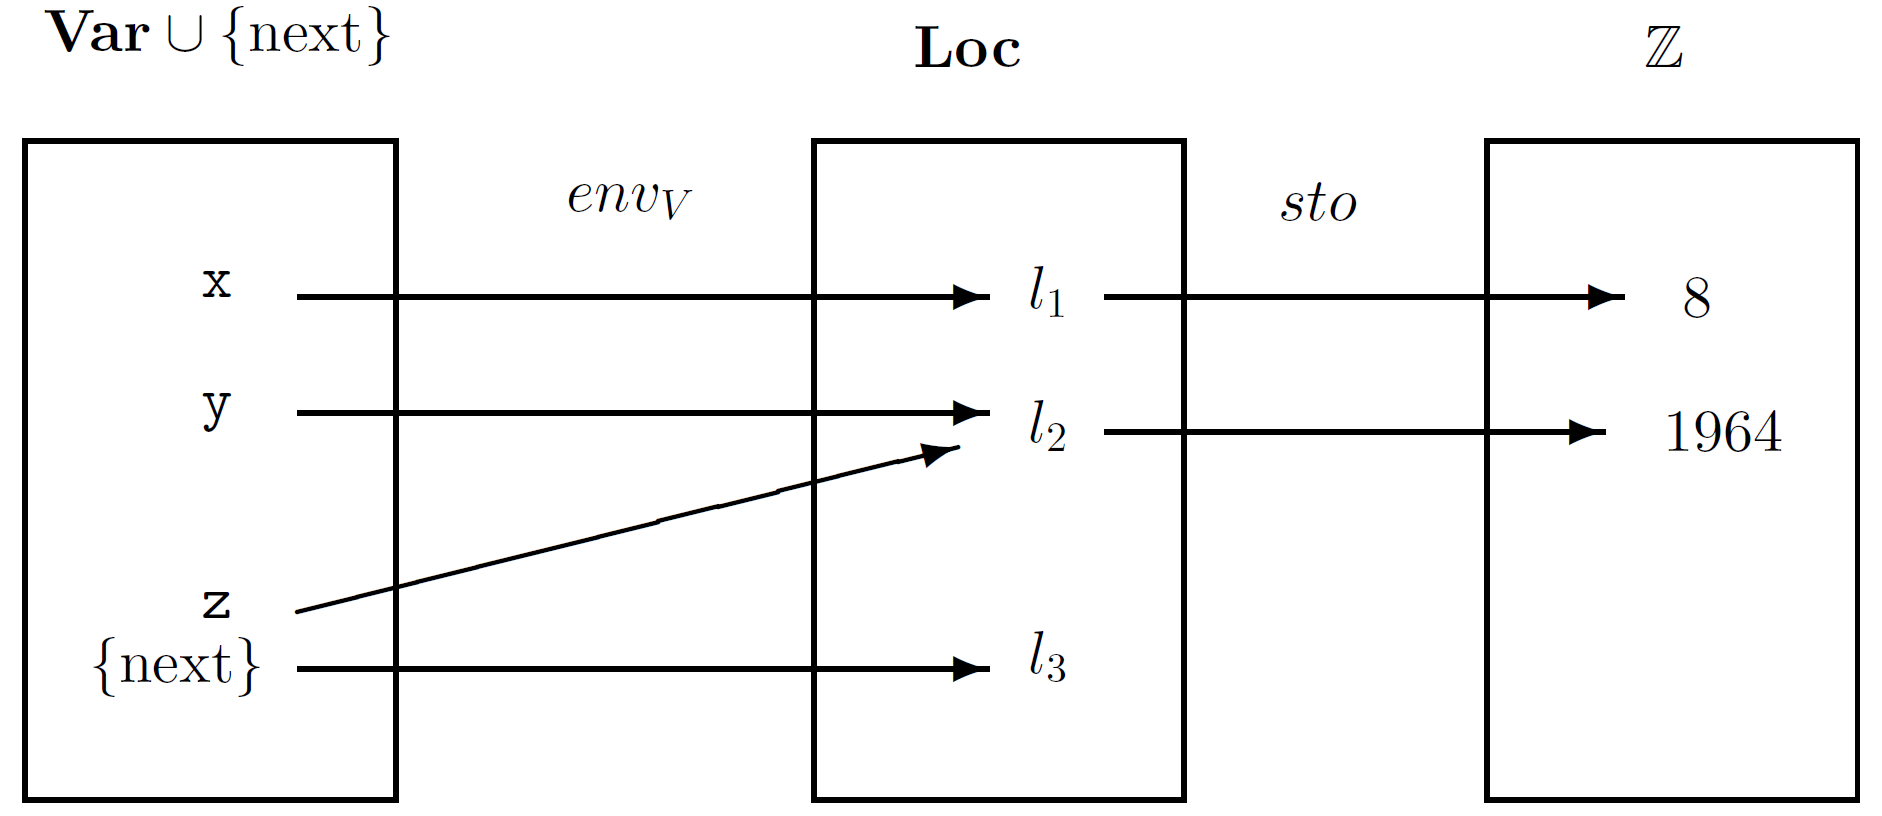
\includegraphics[width=0.8\textwidth]{figures/Environment_Store.png}
    \caption{Example diagram of the environment store model~\cite{Huttel2010}.}
    \label{fig:envstomodel}
\end{figure}


Arc has three environments: the variable environment, the function environment, and the task environment. To describe the semantics of these environments, some function, set and value names must be defined first. These definitions are presented in Table~\ref{tab:setsandfunctions}, and correspond to rules of Arc's \gls{cfg} described mathematically.

Following the standard of~\cite{Huttel2010}, sets are bolded and begins with a capital letter, while elements are not bolded.


\begin{table}[htb!]
    \centering
    \begin{tabular}{l}
        \toprule
        $\textbf{Val} = \textbf{Num} \cup \textbf{Bool} \cup \textbf{Char} \cup \textbf{Array} \cup \textbf{Pin}\ -$ Values                                                        \\
        $\textbf{Pin} = \textbf{PinValues} \times \textbf{Modes}\ -$ Pins are tuples of Arduino pins and modality                                                                  \\
        $\textbf{Array} = \mathbb{N} \rightharpoonup \textbf{Val} \setminus \textbf{Pin}\ -$ Arrays map numbers to non-pin values                                                  \\
        $\textbf{Par} = \textbf{Types} \times \textbf{Var}\ -$ Set of possible formal parameters                                                                                   \\
        $\textbf{Trig} = \{\epsilon, (\text{every} \times \mathbb{N}), (\text{when} \times \textbf{Expr}) \}\ -$ Set of triggers                                                   \\
        $v \in \textbf{Val}\ -$ Literal values                                                                                                                                     \\
        $x \in \textbf{Var}\ -$ Variable id                                                                                                                                        \\
        $f \in \textbf{Fun}\ -$ Function id                                                                                                                                        \\
        $t \in \textbf{Types}\ -$ Type names                                                                                                                                       \\
        $y \in \mathcal{P} (\textbf{Par})\ -$ Formal parameter lists                                                                                                               \\
        $r \in \mathcal{P} (\textbf{Var})\ -$ Reference parameter lists                                                                                                            \\
        $S \in \textbf{Stm}\ -$ Statements                                                                                                                                         \\
        $l \in \textbf{Loc}\ -$ An arbitrary location in \textbf{Loc}                                                                                                              \\
        next $\ -$ A special 'pointer' holding the value of the next element in \textbf{Loc}                                                                                       \\
        new $: \textbf{Loc} \rightarrow \textbf{Loc}\ -$ function to return succesor location                                                                                      \\
        \\
        $\textbf{Sto} = \textbf{Loc} \rightharpoonup \textbf{Val}\ -$ Set of stores                                                                                                \\
        $\textbf{Env}_V = \textbf{Var} \cup \{\text{next}\} \rightharpoonup \textbf{Loc}\ -$ Set of variable environments                                                          \\
        $\textbf{Env}_F = \textbf{Fun} \rightharpoonup \textbf{Stm} \times \mathcal{P} (\textbf{Par}) \times \textbf{Env}_V \times \textbf{Env}_F\ -$ Set of function environments \\
        $\textbf{Env}_T = \textbf{Stm} \times \mathcal{P} (\textbf{Var}) \times \textbf{Trig} \times \textbf{Env}_V \times \textbf{Env}_F\ -$ Set of task environments             \\
        \bottomrule
    \end{tabular}
    \caption{Sets and function definitions.}
    \label{tab:setsandfunctions}
\end{table}

\supervisor{Should we define types as $\{\epsilon, mut\} \times \textbf{Typenames} \cup \textbf{Typenames}$}


Additionally, we define the notation for updating a given environment $env_V \in \textbf{Env}_V$ we write $env_V[ x \mapsto l]$ to denote the update of $env_V$ given by


\begin{equation}
    env_V[x \mapsto l](y) =
    \begin{cases}
        env_V(y) & y \neq x \\
        l        & y = x
    \end{cases}
\end{equation}


\noindent and $env_F[ f \mapsto (S, y, env_V, env_F)]$ for $env_F$


\begin{equation}
    env_F[f \mapsto (S, y, env_V, env_F)](g) =
    \begin{cases}
        env_F(g)             & g \neq f \\
        (S, y, env_V, env_F) & g = f
    \end{cases}
\end{equation}


\noindent and similarly for a $sto \in \textbf{Sto}$ we write $sto[ l \mapsto v ]$ to indicate the update of $sto$ given by


\begin{equation}
    sto[l \mapsto v](l^\prime) =
    \begin{cases}
        sto(l) & l \neq l^\prime \\
        v      & l = l^\prime
    \end{cases}
\end{equation}
\todo{Missing $env_T$ definition. Should just be a set union an element.}

\noindent With the above definitions of the environment store model and the scope rules, Arc's declarations are described using operational semantics in Table~\ref{tab:arcscoperules}. Because of the static scope rules, the environments are contained within the results of the partial functions for variables and functions. Unlike the variable and function environments, the task environment is not a set of partial functions. This is because unlike function declarations, tasks are not used within other tasks, and as such does not need to map them.


\begin{table}[htb!]
    \small
    \centering
    \begin{tabular}{ll}
        \toprule
        $[PIN_{DECL}]$  & $\frac
            {\langle env^{\prime\prime}_V, sto[l \mapsto v] \rangle \rightarrow (env^\prime_V, sto^\prime)}
            {\langle \text{\#pin} \ x = (pv, mode), env_V, sto\rangle\rightarrow (env^\prime_V, sto^\prime)}$ \\ [12pt]
                        & where $(pv, mode) \in \textbf{Pin} $                                                \\
                        & and $(pv,mode) \rightarrow v $                                                      \\
                        & and $l = env_V(\text{next})$                                                        \\
                        & and $env^{\prime\prime}_V = env_V[x \mapsto l][\text{next} \mapsto \text{new}(l)] $ \\
        \\

        $[VAR_{DECL}]$  & $\frac
            {\langle env^{\prime\prime}_V, sto[l \mapsto v] \rangle \rightarrow (env^\prime_V, sto^\prime)}
            {\langle t \ x = expr, env_V, sto\rangle\rightarrow (env^\prime_V, sto^\prime)}$                  \\ [12pt]
                        & where $env_V, sto \vdash expr \rightarrow v $                                       \\
                        & and $l = env_V(\text{next})$                                                        \\
                        & and $env^{\prime\prime}_V = env_V[x \mapsto l][\text{next} \mapsto \text{new}(l)] $ \\
        \\

        $[FUNC_{DECL}]$ & $\frac
            {env_V \vdash \langle env_F[f \mapsto \langle S, y, env_V, env_F\rangle] \rangle \rightarrow env^\prime_F}
            {env_V \vdash \langle t \ f (y) \{S \}, env_F \rangle \rightarrow env^\prime_F}$                  \\ [12pt]

        $[TASK_{DECL}]$ & $\frac
            {env_{VF}\vdash \langle env_T[S, r, trig, env_V, envF] \rangle \rightarrow env^\prime_T}
            {env_{VF}\vdash \langle \text{task} \ (r) trig \{S\} \rangle \rightarrow env^\prime_T}$           \\
        \bottomrule
    \end{tabular}
    \caption{Arc's declarations and effects on scope defined with operational semantics.}
    \label{tab:arcscoperules}
\end{table}


To use the declared bindings we further define their calling and usage. Variables are immutable, and it therefore makes sense to have functions use call-by-value for the parameters. Function calls should not allow recursion, as this makes the runtime memory usage of the Arduino more stable.

Tasks are once again special. They are never called explicitly in Arc code, but the set of all declared tasks serve as the entrypoint of the program. This is done through parallel composition and invocation of all declared tasks, of which there must be at least one.

Also of importance is that the parameters of a task describe a mutable reference to a declared variable in $env_V$, that critically cannot be used in another task. This means that declarations are implicit calls with a call-by-reference model for its parameters.


\begin{table}[htb!]
    \centering
    \begin{tabular}{ll}
        \toprule
        $FUNC_{CALL}$ & $\frac{}{env_{VF} \vdash \langle f(e), sto\rangle \rightarrow sto^\prime}$ \\ [12pt]
                      & where $env_F(f) = \langle S, y, env^\prime_V, env^\prime_F \rangle$        \\
                      & and $\forall i | 0 \leq i \leq |y|$                                        \\
                      & and $e \in \textbf{Expr}^{ |y| }$                                          \\
                      & and $\forall i $                                                           \\

        $ENTRY$       & $\frac{}{}$                                                                \\ [12pt]
        \bottomrule
    \end{tabular}
    \caption{Semantics for function calls and task invocation.}
    \label{tab:callandentry}
\end{table}
\supervisor{How do I describe that each expression in the parameter list is evaluated and stored in a new location, with a variable $y_i$ from the formal parameter list pointing to that location?!}


\subsection{Type rules}\label{subsec:typerules}
Type rules are another set of contextual constraints. These rules make sure that code fragments do not mistreat types, for example in static typing, which Arc uses, it should not be possible to assign a number to a variable declared as a boolean~\cite{Sebesta2016}. The types that are valid in Arc are num, char, bool, and array, as descriped in~\ref{sec:inspiration}.

In the type checking semantics the types in the Arc language can be written as:
$T \in \{num, char, bool, N\} N \in \{ 0,\mathbb{N}\}$.
From now on semantics written mathmatticly will use T instead of type, if not given a specific type, in semantic type checking. If a specific type is needed, it is written instead of T.
N is not descriped ealier on what the types are in Arc, as it is not a type that can be declared. N is used for accessing an array, In C++ array access has to have a natural number, this is also implemented in Arc aswell. In C++ it is also 0-indexed~\cite{cppreferenceDataTypes}, which is withhold in Arc aswell.
In declarations and statements type checking, there will be an evaluation to $ok$ which means:

\blockcquote{Huttel2010}{The type of a declaration or a statement will simply be ok; we say that the declaration or statement is well-typed}

In Table~\ref*{tab:DeclTypeCheck}, the type checking for variables and functions are written. A specific type function declaration, has to type check if the return type is the same type as the declared function type. As task and a void function do not return, these declarations are always well-typed.


\begin{table}[htb!]
    \centering
    \begin{tabular}{ll}
        \toprule
        $[VAR_{DECL}] $  & $\frac{env \vdash expr : T}{env \vdash T \;x = expr : ok}$                            \\  [12pt]
        $[FUNC_{DECL}] $ & $\frac{env \vdash expr : T}{env \vdash T \;f() \{S; \;\text{return} \; expr\}  : ok}$ \\  [12pt]
        $[VOID_{DECL}] $ & $f()\{S\}  : ok$                                                                      \\
        \bottomrule
    \end{tabular}
    \caption{Arc type check for declarations.}
    \label{tab:DeclTypeCheck}
\end{table}


Now that the types has been clarified, it is important to look at operations a specific type can do.
The first type that will be clarified is num.
In Table~\ref{tab:num-rules} the expressions which the data type num only can do, is showed here.


\begin{table}[htb!]
    \centering
    \begin{tabular}{lll}
        \toprule
        $[ADD_{EXPR}] $                         & $\frac
            {env\vdash expr_1: num \quad env\vdash expr_2: num}
            {env\vdash expr_1 \;+\;expr_2: num}$
        \\ [12pt]
        $[SUB_{EXPR}] $                         & $\frac
            {env\vdash expr_1: num \quad env\vdash expr_2: num}
            {env\vdash expr_1 \;-\;expr_2: num}$
        \\ [12pt]
        $[MULT_{EXPR}] $                        & $\frac
            {env\vdash expr_1: num \quad env\vdash expr_2: num}
            {env\vdash expr_1 \;*\;expr_2: num}$
        \\ [12pt]
        $[DIVI_{EXPR}] $                        & $\frac
            {env\vdash expr_1: num \quad env\vdash expr_2: num}
        {env\vdash expr_1 \; / \; expr_2: num}$ & where $expr_2 \neq 0$
        \\ [12pt]
        $[REL_{EXPR}] $                         & $\frac
            {env\vdash expr_1: num \quad env\vdash expr_2: num}
            {env\vdash expr_1 \; OP \; expr_2: Bool}$                                 \\

                                                & where $OP \in \{<, >, \leq, \geq\}$

        \\
        \bottomrule
    \end{tabular}
    \caption{Type rules for num expressions in Arc.}
    \label{tab:num-rules}
\end{table}


The type num is the only type in Arc that can do arithmetic expressions, as it can only do arithmetic expressions on another num type, this can be seen in Table~\ref{tab:num-rules}. The end type of a arithmetic expression is still a num, as it makes changes to the value, not the type.

It is also the only type to check if a value is greater or smaller than an other num type when comparing. When doing a comparing of nums, the end type of the expression is a bool, as it true or false if the num is greater or less than the num it is compared to.


\begin{table}[htb!]
    \centering
    \begin{tabular}{ll}
        \toprule
        $[AND_{EXPR}] $ & $\frac
            {env\vdash expr_1: Bool \quad env\vdash expr_2: Bool}
            {env\vdash expr_1 \;\text{and} \;expr_2: Bool}$
        \\ [12pt]
        $[OR_{EXPR}] $  & $\frac
            {env\vdash expr_1: Bool \quad env\vdash expr_2: Bool}
            {env\vdash expr_1 \;\text{or} \;expr_2: Bool}$
        \\ [12pt]
        $[NOT_{EXPR}] $ & $\frac
            {env\vdash expr_1: Bool}
            {env\vdash \text{not} \; expr_1 : Bool}$
        \\
        \bottomrule
    \end{tabular}
    \caption{Type rules for bool expressions in Arc.}
    \label{tab:bool-rules}
\end{table}


The type bool has three expressions, that can be seen in Table~\ref{tab:bool-rules}. This means in the And, Or or Not expressions the expression getting type checked has to evaluate to a bool, the expressions will then evaluate to another type bool.


\begin{table}[htb!]
    \centering
    \begin{tabular}{ll}
        \toprule
        $[ARRAY_{EXPR}]$      & $ \frac
            {env\vdash expr_1: T \quad env \vdash expr_2 : N}
            {env\vdash expr_1[expr_2] : T}$
        \\ [12pt]
        $[PARENTHESIS{EXPR}]$ & $ \frac
            {env\vdash expr_1: T}
            {env\vdash (expr_1) : T}$
        \\ [12pt]
        $[EQUAL_{EXPR}] $     & $\frac
            {env\vdash expr_1: T \quad env\vdash expr_2: T}
            {env\vdash expr_1 \;== \;expr_2: Bool}$
        \\ [12pt]
        $[NOTEQUAL_{EXPR}] $  & $\frac
            {env\vdash expr_1: T \quad env\vdash expr_2: T}
            {env\vdash expr_1 \;!= \;expr_2: Bool}$
        \\
        \bottomrule
    \end{tabular}
    \caption{Type rules for other types of expressions in Arc.}
    \label{tab:expr-rules}
\end{table}


The type char does not have any expressions that only can be used on that type, therfore it only can use the expressions which bool and num can do as well. These type rules for expressions is written on Table~\ref{tab:expr-rules}. In the array expression the type N is used to describe the index for the array. The equal and not equal expression evaluate to a bool type, as it can only be true or false.


\begin{table}[htb!]
    \centering
    \begin{tabular}{ll}
        \toprule
        $[COMP_{STMT}] $     & $\frac
            {env \vdash stmt_1 :ok \quad env \vdash stmt_2 :ok}
            {env \vdash stmt_1\;;\;stmt_2: ok}$
        \\ [12pt]
        $[VAR-DECL_{STMT}] $ & $\frac
            {env \vdash expr : T}
            {env \vdash  T \;x = expr: ok}$
        \\ [12pt]
        $[ASSIGN_{STMT}]$    & $\frac
            {env\vdash x: T \quad env \vdash expr : T}
            {env\vdash x = expr: ok}$
        \\ [12pt]
        $[INDEX_{STMT}] $    & $\frac
            {env \vdash x : T \quad env \vdash expr : N \quad env \vdash expr : T}
            {env \vdash x[expr] = expr: ok}$
        \\ [12pt]
        $[BLOCK_{STMT}] $    & $\frac
            {env \vdash stmt :ok}
            {env \vdash \{stmt\}: ok}$
        \\ [12pt]
        $[CALL_{STMT}] $     & $\frac
            {env \vdash f:(x:T \rightarrow ok)\quad env \vdash expr:ok}
            {env \vdash call \;f(expr): ok}$
        \\ [12pt]
        $[RETURN_{STMT}] $   & $\frac
            {env \vdash expr: T}
            {env \vdash \text{return} \;expr: ok}$
        \\ [12pt]
        $[IF_{STMT}] $       & $\frac
            {env \vdash if (expr) : Bool \quad env \vdash stmt_1 :ok \quad env \vdash stmt_2 :ok}
            {env \vdash \text{if} (expr) \;stmt_1 \;\text{else} \;stmt_2: ok}$
        \\ [12pt]
        $[WHILE_{STMT}] $    & $\frac
            {env \vdash  expr : Bool \quad env \vdash stmt :ok}
            {env \vdash \text{while} (expr) \;stmt : ok}$
        \\ [12pt]
        $[FOR_{STMT}] $      & $\frac
            {env \vdash  y : T \quad env \vdash x : T \quad env \vdash block :ok}
            {env \vdash \text{for} (y \; \text{in} \; x) \; block : ok}$
        \\
        \bottomrule
    \end{tabular}
    \caption{Arc type check statements.}
    \label{tab:StatementTypeCheck}
\end{table}


The type checking for statements in Arc can be seen in Table~\ref{tab:StatementTypeCheck}. Type checking statements gives the same output as the declarations in "ok", as explained before means well-typed. A varable can be declared in a scope, therfore it has the same type check rules as in variable declaration, which can be seen in Table~\ref{tab:DeclTypeCheck}. Return uses an expression which evaluates to a type "T", this type is the same type as the type a function is declared with.

\chapter{Language semantics}\label{cha:languagesemantics}

Example semantics:

\begin{align*}
    [COMPOSITION] \quad &
    \frac
    {S_1, \sigma \rightarrow \sigma \prime \quad S_2, \sigma \prime \rightarrow \sigma \prime \prime}
    {S_1;S_2, \sigma \rightarrow \sigma \prime \prime}
    \\
    [RULE]     \quad    &
    \frac
    {Premises}
    {Conclusion}
\end{align*}

\begin{align*}
    [RULE]     \quad &
    \frac
    {Premises}
    {Conclusion}
    Side condition
\end{align*}
